\newpage
\section*{\centering Реферат}
\addcontentsline{toc}{section}{Реферат}
Отчет \pageref{LastPage} с., 3 ч., 2 табл., 4 рис., 23 источника.

\textbf{Тема:} Опыты нечеткого прогнозирования.

\textbf{Объектом исследования} являются методы прогнозирования на основе систем нечеткого вывода.

\textbf{Предмет исследования:} точность прогноза по нечетко-логическому методу в одномерном случае на данных социального типа.

\textbf{Цель работы:} выяснение перспектив применения одномерной модели.

\textbf{Поставленные задачи} для достижения цели НИР:
\begin{itemize}
	\item обзор литературы по теме нечеткого прогнозирования социально-экономических процессов.
	\item опытная проверка результатов одномерных нечетко-логических моделей и сравнение с	моделями на основе теории нечетких временных рядов.
\end{itemize}

\newpage
\section*{Введение}
\addcontentsline{toc}{section}{Введение}

Проблема эффективного прогнозирования социально-экономических процессов в настоящее является исключительно актуальной задачей. Особенную сложность прогнозирование приобретает в задачах государственного управления. В силу того, что государственные планы и прогнозы затрагивают жизнь большого числа людей, возрастает цена ошибки. Поэтому необходимо минимизировать риски. Одним из способов минимизации рисков является научный подход в прогнозировании возможных сценариев развития общества.  

Социально-экономическим процессам свойственны неопределенность, наличие скрытых факторов влияния, слабая предсказуемость. Системы, характеризующиеся такими процессами, называют нелинейными, хаотическими, случайными, неопределенными. Существуют математические теории, призванные <<уточнять>> неточности: теория детерминированного хаоса, теория вероятностей, нечеткая логика и др. В данной работе рассматриваются прикладные аспекты социального прогнозирования с помощью нечеткой логики.

\textbf{Цель работы:} выяснение перспектив применения одномерных нечетких моделей.

\textbf{Поставленные задачи} для достижения цели НИР:
\begin{itemize}
	\item обзор литературы по теме нечеткого прогнозирования социально-экономических процессов.
	\item опытная проверка результатов одномерных нечетко-логических моделей и сравнение с	моделями на основе теории нечетких временных рядов.
\end{itemize} 



\newpage
\section{Обзор литературы по нечеткому социальному прогнозированию}

Первые случаи применения теории нечеткой логики связаны с созданием контроллеров для управления техническими системами. Так, в 1987 году в японском городе Сендай была открыта железнодорожная линия, на пассажирских поездах которой были установлены нечеткие системы, регулирующие ускорение, торможение и остановку поезда. С тех пор применение нечетких контроллеров значительно возросло, затрагивая, к примеру, производство бытовой техники (кондиционеры, посудомоечные машины, пылесосы), автомобилестроение (повышение энергоэффективности двигателей), распознавание образов и др.

Однако, перспективы применения нечеткой логики для моделирования и прогнозирования социально-экономических процессов остаются малоизученными. Данный небольшой обзор рассматривает работы по нечеткому прогнозированию с использованием данных государственной статистики. 

В статье  Н. А. Абдуллаевой \cite{Abdullaeva2010} исследуется уровень бедности в Азербайджане в зависимости от доходов населения, коэффициента безработицы, уровня
инфляции и прожиточного минимума, а также дается прогноз
уровня бедности на три года. Для прогноза уровня бедности предлагается нечеткая регрессионная модель. Утверждается превосходство нечеткого регрессионного моделирования перед классическим регрессионным моделированием при прогнозировании уровня бедности, так как оно обеспечивает большую точность результатов. 

Работа М. Г. Мамедовой и З. Г. Джабраиловой \cite{Mamedova2005} 
показывает целесообразность применения нечеткой логики в моделировании демографических аспектов рынка труда на примере задачи прогнозирования численности экономически активного населения. Предложена методика прогнозирования численности экономически активного населения с
использованием модели нечетких временных рядов. Установленный горизонт прогнозирования --- три года. Кроме того, метод применен для долгосрочного прогнозирования (до 2025 года). Проведен сравнительный анализ и интерпретация полученных прогнозных данных для экономически активного, общего и трудоспособного населения, позволившие определить вероятное перспективное состояния рынка труда. 

В статье П. С. Пака и Г. Кима \cite{Pak2005} предлагается основанный на теории нечеткости метод прогнозирования численности и состава населения (пол, возраст, район проживания) на долгосрочный период. На первом этапе представлена нечеткая модель, состоящая из набора правил типа <<если-то>>, для оценки общего роста населения в 402 районах региона Кансай. Антецеденты и консеквенты правил построены с помощью реальных данных, и эти правила составляют нечеткие высказывания и регрессионные модели, соответственно. На втором этапе описан метод для оценки социального роста по полу и возрасту в каждом районе на основе метода нечеткой кластеризации. Метод ориентирован на оценку долгосрочных социоэкономических изменений в миграции населения. Точность результатов предложенной модели сравнивается с традиционной регрессионной моделью, сравнение оказывается в пользу предлагаемой нечеткой модели.   

Исследование А. Сасу \cite{Sasu2010} предлагает методику прогнозирования демографических процессов на основе теории нечетких временных рядов. Своеобразная особенность модели заключается в её способности прогнозировать требуемый показатель, используя неполные, нечеткие входные данные. Автор утверждает возможность установки практически неограниченного горизонта прогнозирования для данной модели.  

Суммируя информацию из рассмотренных источников, заметим некоторые тенденции:
\begin{itemize}
	\item Более высокая точность нечетких моделей в сравнении с классическими моделями для социального прогнозирования.
	\item Широкий диапазон горизонтов прогнозирования: возможность краткосрочного, среднесрочного, долгосрочного прогнозирования.
	\item Разнообразие сценариев применения нечетких моделей для социально-экономических прогнозов.
\end{itemize}
\section{Теорема о нечеткой аппроксимации}

В 1994 году Б. Коско  доказал теорему о нечеткой аппроксимации (Fuzzy Approximation Theorem) \cite{Kosko1994}, согласно которой, любая математическая система может быть аппроксимирована системой на нечеткой логике. Следовательно, с помощью естественно-языковых высказываний <<если-то>>, с последующей их формализацией средствами теории нечетких множеств, можно сколько угодно точно отразить произвольную взаимосвязь <<входы-выход>> без использования сложного аппарата дифференциального и интегрального исчислений, традиционно применяемого в управлении и идентификации. Практические успехи нечеткого управления получили теоретическое обоснование. 

\begin{theorem}[Теорема о нечеткой аппроксимации]
	\label{theorem:FAT}
	Аддитивная нечеткая система  $F$ равномерно аппроксимирует $f: X\rightarrow Y$, если множество $X$ компактно и $f$ непрерывна.
\end{theorem}

\section{Вычислительный эксперимент нечеткой авторегрессии}

\subsection{Используемые программные средства}

В настоящей статье программная реализация методов нечеткого прогнозирования
базируется на библиотеке <<frbs>> языка статистического программирования R. Библиотека разработана докторами философии и аспирантами Гранадского университета. В библиотеке реализовано более 15 методов нечеткой классификации и регрессии. В библиотеке рассматриваются системы с многими входами и единым выходом (MISO) с данными в виде вещественных чисел.

СНВ --- система нечеткого вывода.
\begin{enumerate}
\item СНВ, основанные на разбиении области определения.
\begin{itemize}
\item Метод Ванга и Менделя. Предназначен для решения задач регрессии \cite{Wang1992}.
\item Метод Чи. Предназначен для решения задач классификации \cite{Chi1996}.
\item Взвешенный метод Ишибучи. Предназначен для решения задач классификации \cite{Ishibuchi2001}.
\end{itemize}
\item СНВ, основанные на искусственных нейронных сетях.
\begin{itemize}
	\item Адаптивная нечеткая система вывода с использованием нейросети. Предназначена для решения задач регрессии \cite{Jan1993}. 
	\item Гибридная нечеткая система вывода с использованием нейросети.  Предназначена для решения задач регрессии \cite{Kim1999}.
\end{itemize}
\item СНВ, основанные на алгоритмах кластеризации.
\begin{itemize}
	\item Субтрактивная кластеризация и метод нечеткой кластеризации c-средних.
	Предназначена для решения задач регрессии \cite{Chiu1996}.
	\item Динамическая эволюционирующая система вывода с использованием нейросети. Предназначена для решения задач регрессии \cite{Kasabov2002}.
\end{itemize}	
\item СНВ, основанные на генетических алгоритмах.
\begin{itemize}
	\item Метод Трифта. Предназначен для решения задач регрессии \cite{Thrift1991}.
	\item Генетическая нечеткая система для обучения нечетких правил, основанная на технологии MOGUL. Предназначен для решения задач регрессии \cite{Cordon1999}.
	\item Метод Ишибучи, основанный на генетическом кооперативно-кон\-курентном обучении. Предназначен для решения задач классификации \cite{Ishibuchi1999}.
	\item Метод Ишибучи, основанный на гибридизации генетического ко\-оперативно-конкурентного обучения и Питтсбургского метода. 
	 Предназначен для решения задач классификации \cite{Ishibuchi2005}.
	\item Структурный обучающий алгоритм на нечеткой среде.  
	Предназначен для решения задач классификации \cite{Gonzalez2001}. 
	\item Генетический алгоритм для латеральной настройки и выбора правил лингвистической нечеткой системы. 
	Предназначен для решения задач регрессии \cite{Alcala2007}.
\end{itemize}
\item СНВ, основанные на методе градиентного спуска.
\begin{itemize}
	\item СНВ с использованием эвристик и градиентного спуска. Предназначена для решения задач регрессии \cite{Ishibuchi1994}.
	\item Правила нечеткого вывода по методу спуска. 
	Предназначен для решения задач регрессии \cite{Nomura1992}. 
\end{itemize}
\end{enumerate}

\subsection{Методика проведения эксперимента}

Основными направлениями нечеткого прогнозного моделирования, описанными в литературе, являются теория нечеткой логики \cite{Zadeh1973} и теория нечетких временных рядов \cite{Song1993}.
При этом, для прогнозирования по методу нечетких временных рядов исследователям удалось добиться существенного снижения погрешности прогнозов даже для авторегрессионного случая. 

Известно \cite{sep-principia-mathematica}, что до некоторых пределов математика сводима к логике. Это и будет исходной точкой нашего эксперимента. Попробуем сравнить доказанные в своей успешности методы теории нечетких временных рядов (основанные на математической теории нечетких множеств) с методами нечеткой логики, реализованными в пакете <<frbs>>.  

Объектом прогнозирования являются данные по поступившим в университет Алабамы абитуриентам за период 1971-1992 гг. (см. Рис.~\ref{figure:UA_enrollments}). Именно они были использованы в статье, впервые описавшей теорию нечетких временных рядов и с тех пор являются основой для сравнения моделей.  

\begin{figure}[bhtp]
	\begin{center}			
		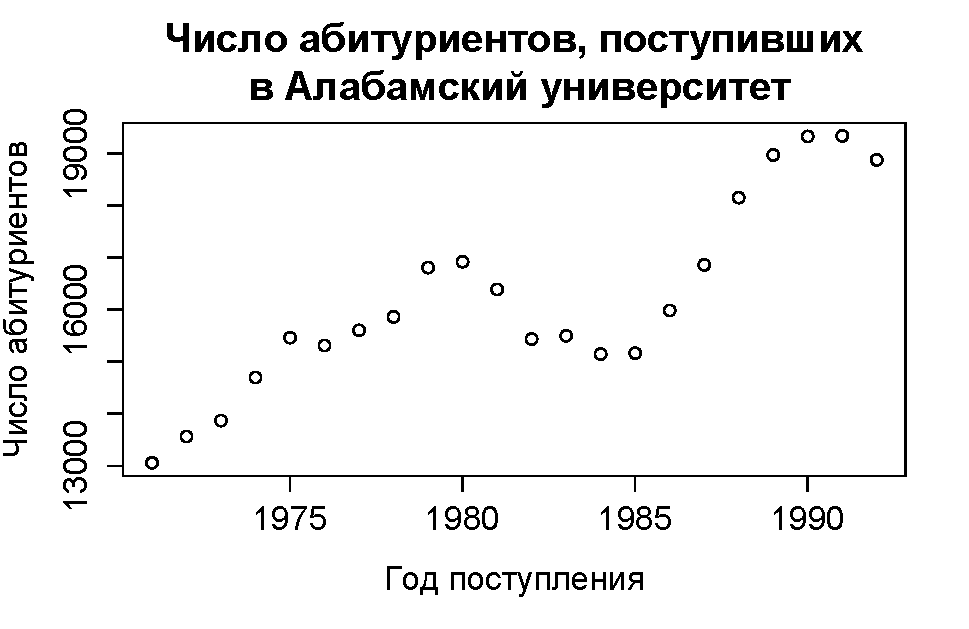
\includegraphics{images/UA_enrollments.pdf}
		\caption{Число поступивших в Алабамский университет, 1971-1992.}		
		\label{figure:UA_enrollments}
	\end{center}
\end{figure}

По итогам экспресс-теста регрессионных моделей решено было выбрать модель авторов Л-Х. Ванга и Дж. М. Менделя, основанную на разбиении области определения \cite{Wang1992}. Критериями отбора были точность прогноза на тестовых данных и сложность вычислений. Модель демонстрирует хорошую точность и низкую вычислительную сложность. 

Алгоритм Ванга и Менделя состоит из пяти шагов:
\begin{enumerate}
	\item Разбиение областей определения входных и выходных численных данных на нечеткие интервалы.
	\item Генерация нечетких правил на основе предоставленных данных.
	\item Присвоение степени каждому из сгенерированных правил с целью разрешения противоречий между правилами.
	\item Создание комбинированной нечеткой базы правил, основанной одновременно на 1) автоматически сгенерированных правилах и
	   2) правилах на естественном языке, предложенных экспертами.
	
	\item Определение отображения входного пространства на выходное, основываясь на комбинированной базе правил, с помощью процедуры дефаззификации.
\end{enumerate}

Доказана возможность предлагаемого отображения аппроксимировать любую непрерывную функцию вещественного переменного на компактном множестве с произвольной точностью.
Примеры нечетких правил и функций принадлежности, генерируемых моделью, см. на
Табл.~\ref{table:fuzzy_rules_example} и Рис.~\ref{figure:MFexample}, соответственно.  

\renewcommand{\arraystretch}{1.5} %Space between rows
\setlength{\tabcolsep}{8pt} %Space between columns

\begin{table}[bhtp]
	\caption{Пример нечетких правил.}
	\begin{center}
		\begin{tabular}{ | c | c | }
			\hline
			1 & IF tminus2 is  v.1\_a.1 and tminus1 is  v.2\_a.1 THEN   t  is  c.1 \\
			\hline
			2 & IF tminus2 is  v.1\_a.7 and tminus1 is  v.2\_a.7 THEN   t  is  c.5  \\
			\hline
			\multicolumn{2}{ |c| }{\ldots} \\
			\hline
			17 & IF tminus2 is  v.1\_a.9 and tminus1 is  v.2\_a.6 THEN   t  is  c.7 \\
			\hline
		\end{tabular}		
	\end{center}
	\label{table:fuzzy_rules_example}	
\end{table}

\begin{figure}[bhtp]
	\begin{center}
		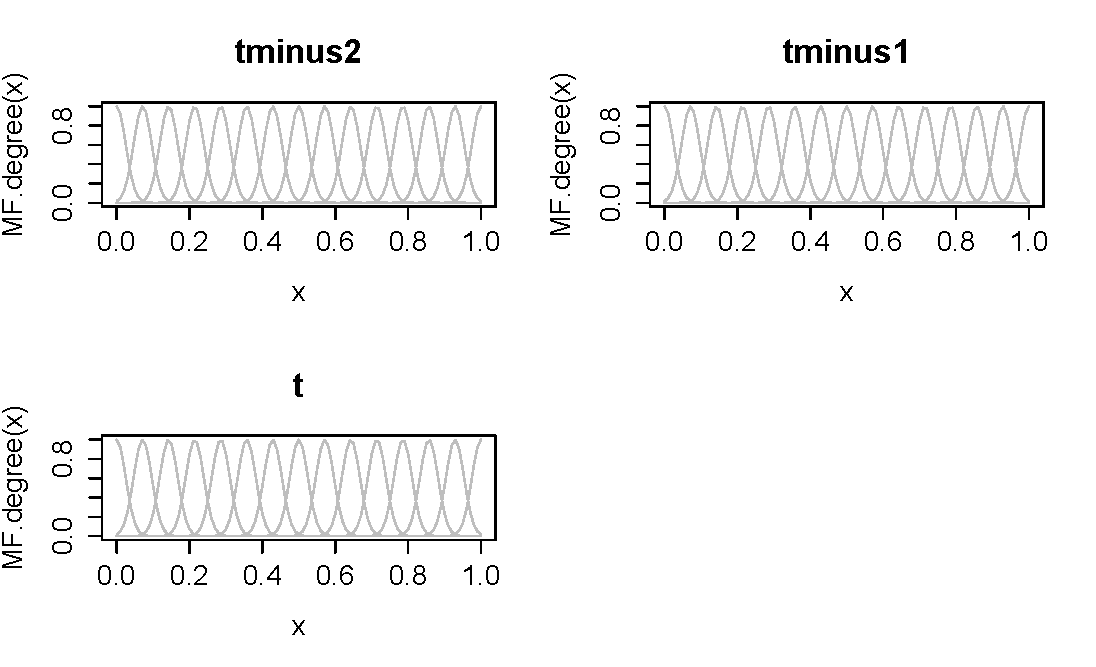
\includegraphics[scale=0.8]{images/MFexample.pdf}
		\caption{Пример функций принадлежности для лингвистических переменных.}		
		\label{figure:MFexample}
	\end{center}
\end{figure}

На выходе модели --- численность поступивших в университет Алабамы за период 1971-1992 гг. ($t$). На входе --- эта же переменная, но со сдвигом на один ($tminus1$) и два ($tminus2$) года назад, соответственно. Таким образом реализована импровизированная авторегрессия по переменной $t$. 

Аналогичным образом в тестовых примерах библиотеки <<frbs>> прогнозировались хаотические временные ряды Маки-Гласса, при этом, однако, сдвиг происходил на 4 и 8 позиций назад и общее число наблюдений составляло 300, а не 22, как в случае с временным рядом поступивших в университет Алабамы.

Общее множество данных разбивалось на два подмножества --- данные для обучения модели и данные для сравнения результатов работы модели --- в зависимости от величины горизонта прогнозирования. 

\subsection{Результаты эксперимента}

В эксперименте использовались два значения горизонта прогнозирования --- 5 лет (см. Рис.~\ref{figure:UA_model_h=5}) и 3 года (см. Рис.~\ref{figure:UA_model_h=3}). Заметим, что в обоих случаях симуляция в области данных для обучения сработала достаточно хорошо, несмотря на крайне малый объем выборки. 

\begin{figure}[bhtp]
	\begin{center}
		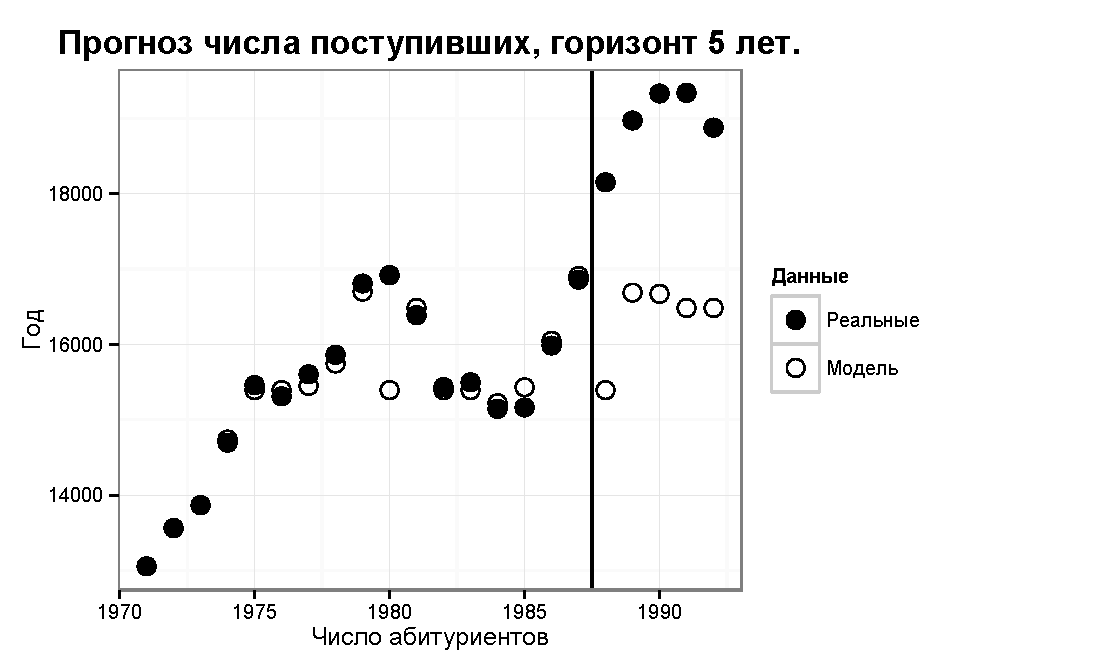
\includegraphics{images/UA_model_h=5.pdf}
		\caption{Прогноз числа поступивших в Алабамский университет, \newline горизонт 5 лет.}		
		\label{figure:UA_model_h=5}
	\end{center}
\end{figure}

\begin{figure}[bhtp]
	\begin{center}
		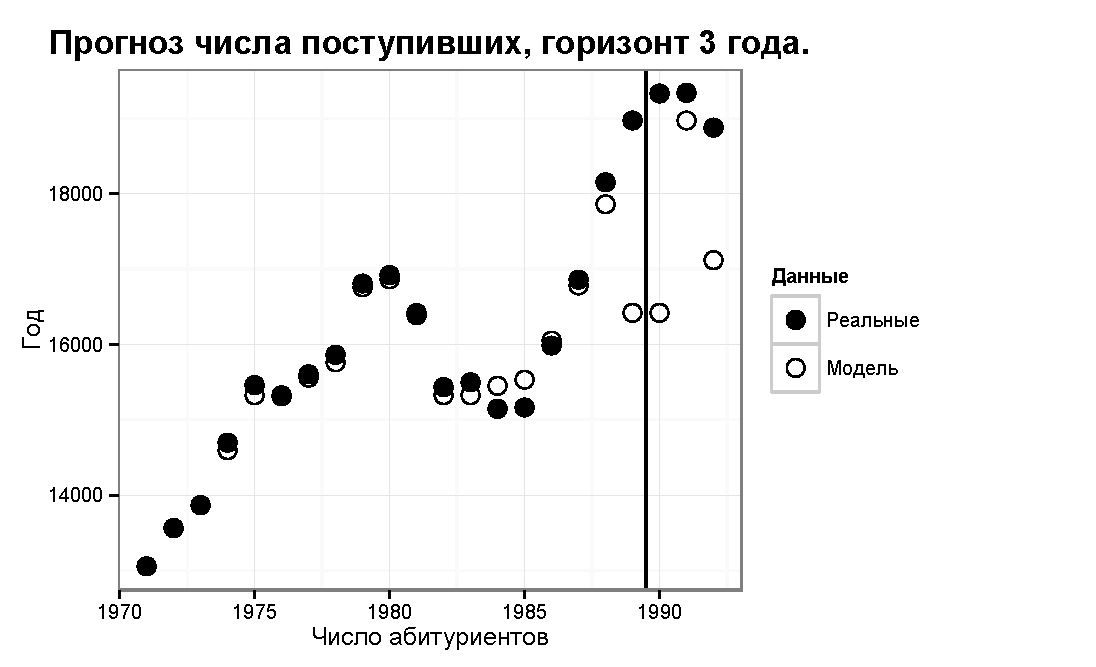
\includegraphics{images/UA_model_h=3.pdf}
		\caption{Прогноз числа поступивших в Алабамский университет, \newline горизонт 3 года.}		
		\label{figure:UA_model_h=3}
	\end{center}
\end{figure}

В части прогноза же результаты неудовлетворительные. Это подтверждается и оценкой погрешности прогнозирования (см. Табл.~\ref{table:WM-error}). Погрешность гораздо выше, чем при авторегрессии методами нечетких временных рядов. С другой стороны, точность увеличивается при уменьшении горизонта прогнозирования. Это говорит о том, что модель адаптируется при изменении параметров и входных данных. 

\begin{table}[bhtp]
	\caption{Оценка точности результатов прогнозирования.}
	\begin{center}
		\begin{tabular}{ | c | c | c | c | }
			\hline
			Горизонт & MSE & RMSE & SMAPE \\
			\hline
			5 & 6.750612e+06 & 2.598194e+03 & 3.674307e+00  \\
			\hline
			3 & 3.897863e+06 & 1.974301e+03 & 2.330708e+00  \\
			\hline
		\end{tabular}		
	\end{center}
	\label{table:WM-error}	
\end{table}

Основной причиной низкой точности прогноза, по нашему предположению, является недостаточность исходных данных. Расширение доступной для модели информации с целью повышения качества прогноза может происходить по трем направлениям:
\begin{itemize}
	\item Увеличение объема выборки (периода, который охватывает временной ряд).
	\item Увеличение количества продукционных правил либо изменение существующих правил.
	\item Увеличение количества либо изменение структуры входных показателей, отбор наиболее релевантных задаче показателей.
\end{itemize}

В процессе вычислительного эксперимента автор столкнулся с техническими трудностями:
\begin{itemize}
	\item Невозможность оценки всех моделей из библиотеки <<frbs>> с варьированием всех параметров моделей ввиду нехватки вычислительных мощностей.
	\item Сложность доступа к данным.  
\end{itemize}
	


\newpage
\section*{Заключение}
\addcontentsline{toc}{section}{Заключение}
В работе был проведен обзор литературы, описывающей практическое применение нечетких моделей для социально-экономического прогнозирования. Характерна тенденция положительных результатов, улучшения точности в сравнении с классическими методами.

Приведена теорема, доказывающая, что нечеткие системы являются универсальными аппроксиматорами. Данное утверждение позволяет с уверенностью смотреть на будущее применения нечетких моделей.

Экспериментальная часть данного исследования была направлена на сравнение нечетко-логического и теоретико-множественного (теория нечетких временных рядов) подходов на примере авторегрессии по одной переменной. Согласно результатам эксперимента, нечетко-логический подход показал неудовлетворителньые резуьтаты на заданных данных. Приведены варианты разрешения этой трудности.

Приоритетными направлениями дальнейшей деятельности являются:
\begin{itemize}
	\item Анализ предметной области <<Наркоситуация в Санкт-Петербурге>> с целью выделения релевантных показателей для прогнозирования.
	\item Использование API информационно-аналитической системы <<Антинар>> для упрощения доступа к данным государственной статистики.
	\item Создание графического интерфейса пользователя (предположительно с помощью библиотеки Shiny) с тем, чтобы обеспечить возможность использования моделей более широким кругом пользователей.
	 
	
\end{itemize}

